\section{Fehlerrechnung}

Die einzelnen Intensit\"aten $I_{0,n}$ von allen Messungen sind in der Abbildung
\ref{fig:intensitaet_fit}  zu sehen. Sie wurden gefittet,  und  somit  kann  die
"richtige" Intensit\"at $I_0$  angen\"ahert  werden.  Aus  dem Fit ist zu lesen:

\begin{align*}
    I_0 &= 152.541 \pm 0.265\SI{}{\lumen\per\square\meter} \\
\end{align*}

\begin{figure}[H]
    \centering
    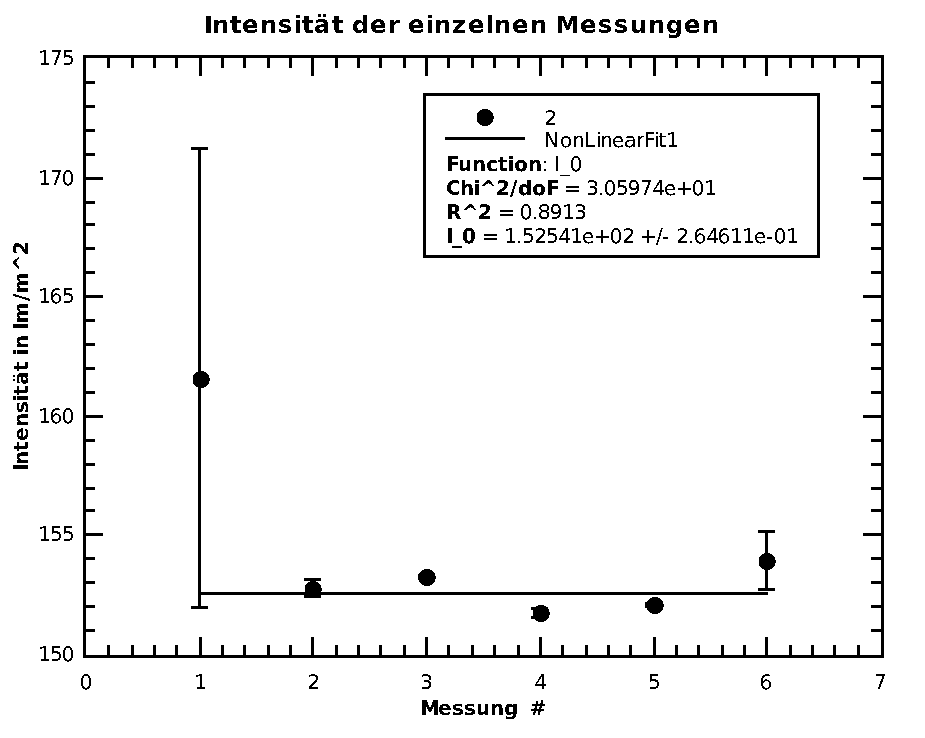
\includegraphics[width=.5\linewidth]{images/intensitaet_fit.pdf}
    \caption{Die einzelnen Intensit\"aten $I_0$ aller Messungen}
    \label{fig:intensitaet_fit}
\end{figure}

Es besteht  ein  unbekannter  Winkel-Offset zwischen Polarisator und Analysator,
bzw. die Winkelanzeige am Pr\"azisionsdrehhalter am Polarisator entspricht nicht
genau der Winkel, der effektiv wirkt. Es kann sein, dass die Primse ein bisschen
daneben liegt. Das gleiche gilt f\"ur den Analysator.

In jeder  Messung  wurden  die  Offsets  gefittet.  Diese  sind in der Abbildung
\ref{fig:offset_fit}  zusammengefasst   und  wurden  gefittet.  Somit  kann  der
``richtige''  Offset  angen\"ahert   werden.   Aus   dem   Fit   ist  zu  lesen:

\begin{align*}
    \varphi_{offset} = 4.7593 \pm 0.0421\SI{}{\degree}
\end{align*}

\begin{figure}[H]
    \centering
    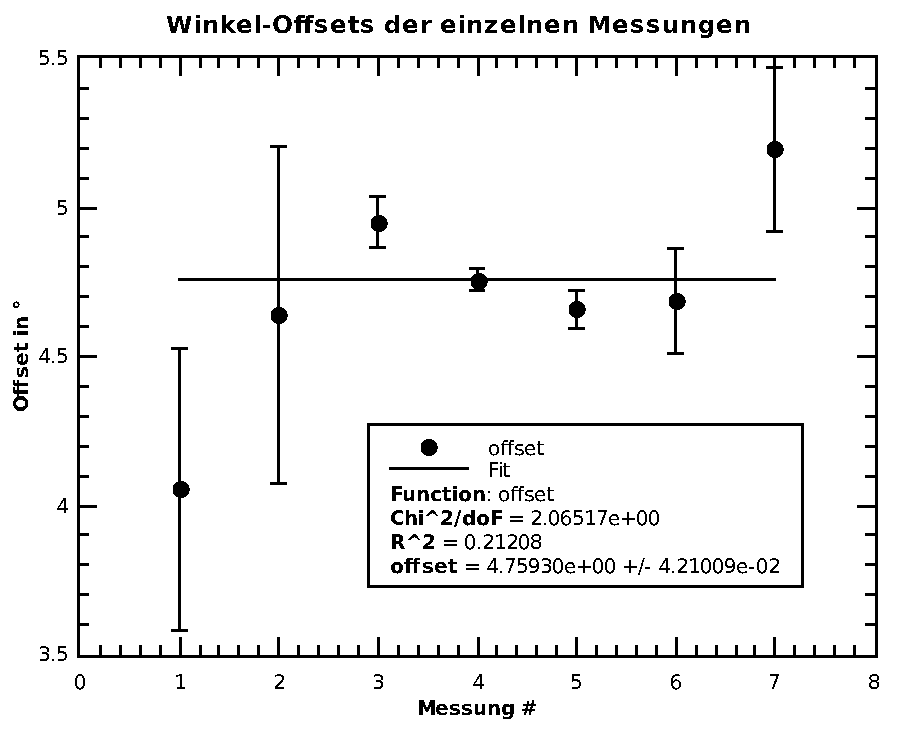
\includegraphics[width=.5\linewidth]{images/offset_fit.pdf}
    \caption{Die einzelnen Offsets $\varphi_{offset}$ aller Messungen}
    \label{fig:offset_fit}
\end{figure}

In der Abbildung \ref{fig:intensitaet_fit} stammen die  Messungen  $2-6$ von der
Aufgabe 5. Da war  die  Frage: ``\textit{Ist $I_0$ in guter N\"aherung konstant,
worauf k\"onnten Abweichungen zur\"uckgef\"uhrt werden?}''.

Die  Antwort  auf  diese  Frage  ist,  dass  einerseits  zuf\"allige  Messfehler
vorliegen,  anderseits  aber  systematische  Fehler,  die  von den Polarisatoren
stammen. In der ersten Messaufgabe,  Abbildungen  \ref{fig:aufgabe-3_falsch} und
\ref{fig:aufgabe-3}, ist  zu  sehen,  dass  die Intensit\"at anders ist wenn der
Analysator \SI{180}{\degree} gedreht ist als wenn  sie  \SI{0}{\degree}  gedreht
ist. Da der Laser  nicht  genau  durch  die  Mitte  des  Polarisators geht, (und
vielleicht  ist  die  Oberfl\"ache  der  Prismen  ein  bisschen  dreckig?),  ist
anzunehmen,  dass  eine  systematische  Abweichung  vorliegt,  in  Funktion  des
eingestellten Winkels.

\begin{figure}[H]
    \centering
    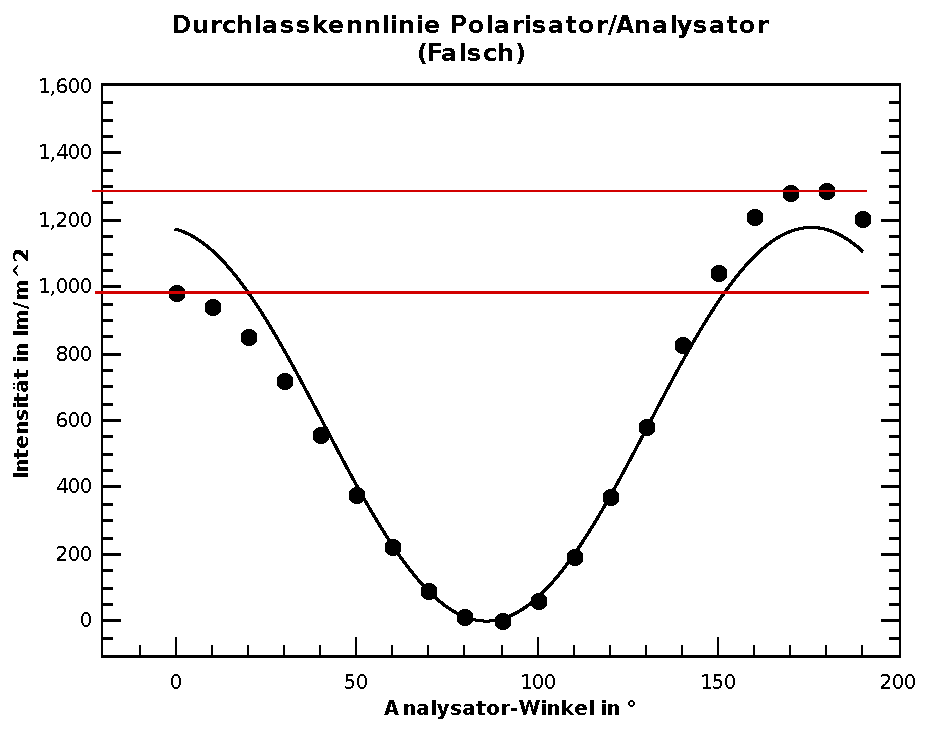
\includegraphics[width=.5\linewidth]{images/intensitaet_sys.pdf}
    \caption{Abweichung Intensit\"at bei \SI{0}{\degree} und \SI{180}{\degree}}
    \label{fig:intensitaet_sys}
\end{figure}

In  der  Abbildung  \ref{fig:intensitaet_sys}   werden   die   Peaks  verglichen
miteinander.         Die         Differenz          betr\"agt         ungef\"ahr
$1290-990=\SI{300}{\lumen\per\square\meter}$

Mit dem Dreisatz  kann  der  Fehler  auf die zweite Messung, wo die Intensit\"at
kleiner    ist,    transformiert   werden.   Der   systematische   Fehler   ist:

\begin{equation}
    s_{I_{0,sys}} = \frac{I_0\cdot\frac{300}{2}}{\frac{1290+990}{2}} = \SI{19.7368}{\lumen\per\square\meter}
\end{equation}

Der totale Fehler ist somit:

\begin{equation}
    s_{I_{0,tot}} = \sqrt{s_{I_{0,sys}}^2 + s_{I_{0,stat}}^2} = \SI{19.739}{\lumen\per\square\meter}
\end{equation}

Und die Intensit\"at $I_0$ ist somit:

\begin{equation}
    I_0 = \overline{I_0} \pm s_{I_{0,tot}} = 152.541 \pm 19.739\SI{}{\lumen\per\square\meter}
\end{equation}

